\chapter{Robert Miller: Reputation, Cashflow, and the Cost of Value}

This School of Hard Knocks interview with Robert Miller opens with the result before the mechanism: companies can close, partners can change, offers can become obsolete, and yet reputation can keep compounding. The chapter follows that order. We begin with the distinction between capital gains and cashflow, move through marketing, sales, finance, and personal brand, and then return to crypto, debt, self-education, relationships, health, and the question of what wealth is finally for. The curation for this companion text is by LazyingArt LLC through Video2Book.

\section{From Capital Gains to Cashflow}

The opening teaser gives us the end of the argument before the beginning. Robert says that with his first agency he was also building a personal brand. The agency shut down. A second agency shut down as well. Then, in his account, the third business scaled to multiple seven figures within about six months because the personal brand had already been built. A newer business was already at a seven-figure runway within roughly sixty days.

The interview then backs up. Robert locates himself in three domains: digital marketing, e-commerce, and crypto. He says he entered crypto young, around age seventeen or eighteen, and places the starting period around 2015--2016. The first conceptual pivot comes when he explains that he had made some money in crypto before taking a digital marketing course, but that money was not yet a business.

\begin{equation}
\hbox{capital gains} \neq \hbox{cashflow}.
\end{equation}

This is the first hinge. A rising asset can produce a gain, but a gain is not the same thing as an operating engine. In the most ordinary accounting language,

\begin{equation}
\hbox{cashflow} = \hbox{cash in} - \hbox{cash out}.
\end{equation}

Robert's point is not that capital gains are unimportant. The early crypto gain gave him capital, confidence, and a story. But it did not yet give him a repeatable mechanism for acquiring customers, selling, delivering, and understanding the movement of money. That is why the narrative moves from crypto into digital marketing.

\subsection{Question \& Answer}

\paragraph{Question.} Why were crypto gains not enough?

\paragraph{Answer.} Because, in Robert's framing, crypto gains were capital gains rather than cashflow. A position can rise in value and still leave the operator without a repeatable business. The missing mechanism was the ability to create demand, convert that demand into sales, and manage the resulting cash. The lesson is not anti-crypto; it is pro-operating discipline.

\section{Scaling as Marketing, Sales, and Finance}

Once the interview asks about scaling a business, Robert gives a sequence rather than a slogan. First comes marketing: not merely paid ads, but content, traffic, and the practical problem of getting people to care about what one says and does. He names Facebook, TikTok, Instagram, and YouTube as attention channels.

Second comes sales. Leads are not yet revenue. A weak salesperson with many leads may still get something, but Robert's stronger claim is that good marketing plus good sales can create fast growth. Third comes finance, which he calls a little unconventional in this context: understanding how the cashflows work.

A compact reconstruction of the growth mechanism is

\begin{equation}
R \approx L \cdot c \cdot P,
\end{equation}

where \(R\) is revenue, \(L\) is leads or traffic, \(c\) is the conversion or close rate, and \(P\) is average purchase or contract value. Robert does not present this formula. It is our notation for the order of his claim: attention creates leads, sales converts leads, and finance tells us whether the revenue is actually strengthening the business.

\begin{figure}
\centering
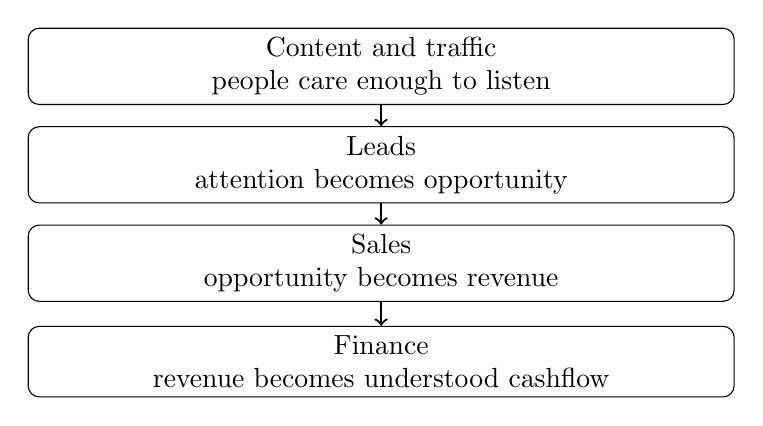
\begin{tikzpicture}[
  box/.style={draw, rounded corners, align=center, text width=0.72\linewidth, minimum height=0.58cm},
  arr/.style={->, thick}
]
\node[box] (a) at (0,0) {Content and traffic\\people care enough to listen};
\node[box] (b) at (0,-1.25) {Leads\\attention becomes opportunity};
\node[box] (c) at (0,-2.50) {Sales\\opportunity becomes revenue};
\node[box] (d) at (0,-3.75) {Finance\\revenue becomes understood cashflow};
\draw[arr] (a) -- (b);
\draw[arr] (b) -- (c);
\draw[arr] (c) -- (d);
\end{tikzpicture}
\end{figure}

The important feature is the ordering. The interview does not start from a spreadsheet. It starts from market attention, then conversion, then financial clarity.

\section{Frameworks Before Tactics}

The book question slows the pace and shows how Robert imports operating frameworks. He names three books, each attached to a different business function.

\begin{table}
\centering
\begin{tabular}{|p{0.30\linewidth}|p{0.60\linewidth}|}
\hline
\emph{The Road Less Stupid} & Strategic thinking before launching a product, offer, or plan. \\
\hline
\emph{Multipliers} & Team leverage, alignment, and multiplying other people's efforts. \\
\hline
\emph{Predictable Revenue} & Sales structure and predictable revenue generation. \\
\hline
\end{tabular}
\end{table}

The list is not incidental. It gives the chapter a middle layer between raw tactics and durable wealth: think clearly, multiply people, then build a revenue machine. That order prepares the next point, because a business machine can be rebuilt only if something durable survives the old machine's failure.

\section{The Personal Brand as a Durable Asset}

Robert then returns to the opening puzzle. Businesses in marketing and e-commerce do not necessarily last. Mechanisms change. Offers change. The way one gets sales changes. But the personal brand, in his account, does not disappear in the same way.

Let \(B_t\) denote reputation capital at time \(t\). A cautious way to write the mechanism is

\begin{equation}
B_{t+1}
=
B_t
+
\hbox{public proof of work}
+
\hbox{market trust}
-
\hbox{reputation damage}.
\end{equation}

This is not a measured equation from the interview. It is a compact form of Robert's claim. The business vehicle can fail while the market's memory of the operator persists.

\begin{figure}
\centering
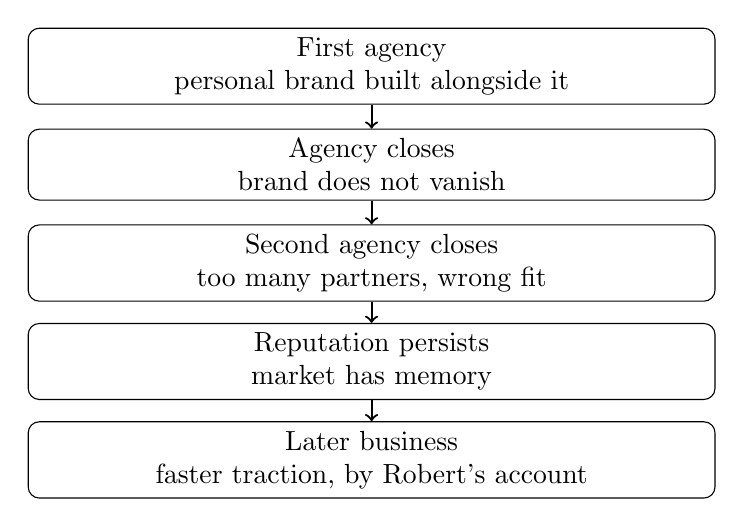
\begin{tikzpicture}[
  box/.style={draw, rounded corners, align=center, text width=0.70\linewidth, minimum height=0.58cm},
  arr/.style={->, thick}
]
\node[box] (a1) at (0,0) {First agency\\personal brand built alongside it};
\node[box] (a2) at (0,-1.25) {Agency closes\\brand does not vanish};
\node[box] (a3) at (0,-2.50) {Second agency closes\\too many partners, wrong fit};
\node[box] (a4) at (0,-3.75) {Reputation persists\\market has memory};
\node[box] (a5) at (0,-5.00) {Later business\\faster traction, by Robert's account};
\draw[arr] (a1) -- (a2);
\draw[arr] (a2) -- (a3);
\draw[arr] (a3) -- (a4);
\draw[arr] (a4) -- (a5);
\end{tikzpicture}
\end{figure}

\subsection{Question \& Answer}

\paragraph{Question.} What survived when the companies did not?

\paragraph{Answer.} Robert's answer is reputation: the personal brand, trust in the market, accumulated attention, and proof that he could acquire clients and execute in digital marketing. In his telling, this durable asset helped a later business reach multiple seven figures in about six months and helped another reach a seven-figure runway within roughly sixty days.

\section{Partners, Failure, and Captive Risk}

The failure section begins with a practical bound. Robert says that one needs about two to three people at most in a partnership or company, not four or five. We should not treat this as a universal theorem, but it is a clear operating rule from his experience:

\begin{equation}
n_{\mathrm{partners}} \approx 2\hbox{--}3,
\qquad
n_{\mathrm{partners}} = 4\hbox{--}5
\quad
\hbox{is risky in this account.}
\end{equation}

The deeper lesson is not arithmetic. It is execution and control. A name means little if nobody executes. An offer means little if nobody executes. A founder can overvalue an idea because it is his idea, but Robert pushes value toward the people who carry the work.

\begin{figure}
\centering
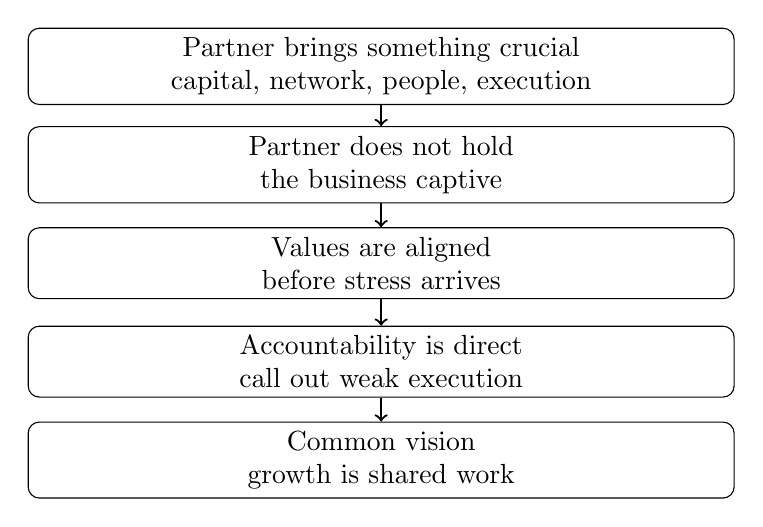
\begin{tikzpicture}[
  box/.style={draw, rounded corners, align=center, text width=0.72\linewidth, minimum height=0.58cm},
  arr/.style={->, thick}
]
\node[box] (p1) at (0,0) {Partner brings something crucial\\capital, network, people, execution};
\node[box] (p2) at (0,-1.25) {Partner does not hold\\the business captive};
\node[box] (p3) at (0,-2.50) {Values are aligned\\before stress arrives};
\node[box] (p4) at (0,-3.75) {Accountability is direct\\call out weak execution};
\node[box] (p5) at (0,-5.00) {Common vision\\growth is shared work};
\draw[arr] (p1) -- (p2);
\draw[arr] (p2) -- (p3);
\draw[arr] (p3) -- (p4);
\draw[arr] (p4) -- (p5);
\end{tikzpicture}
\end{figure}

Robert's partner rule has two sides. The partner must be crucial to the business function: capital, connections, people, execution, or network. But the partner must not be able to hold the company captive. Values alignment matters because stress reveals the true arrangement. The interview's language is direct: if one person is slacking, the other should be able to call it out, and both should return to the shared vision.

\section{Crypto, Energy, and the Question of Value}

The cryptocurrency section broadens the discussion from business mechanics to money itself. Robert says crypto is not merely new technology; it is a new way to think about money. He brings in central banks, CBDCs, storage of wealth, scarcity, mining, electricity, and the question of what society treats as valuable.

The local conceptual obstacle is precise: is value simply rarity, or does cost matter? Robert's Bitcoin example is that mining requires facilities, machines, electricity, and transaction verification. His gold example is that a gold bar also has to be mined. We can represent the analogy as

\begin{align}
\hbox{Bitcoin verification}
&\longleftarrow
\hbox{machines}
+
\hbox{electricity}
+
\hbox{mining facility},
\\
\hbox{gold bar}
&\longleftarrow
\hbox{mining}
+
\hbox{energy}
+
\hbox{extraction cost}.
\end{align}

This is not a proof that energy determines value. It is Robert's valuation intuition. The claim is that society may value scarce things partly because real cost, verification, or energy has gone into them.

\begin{figure}
\centering
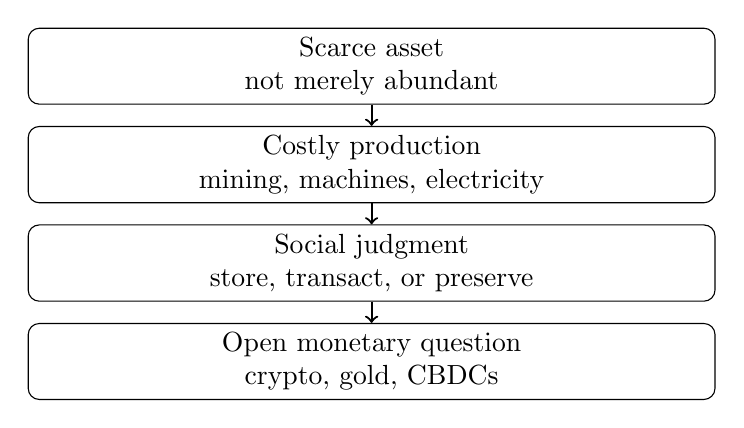
\begin{tikzpicture}[
  box/.style={draw, rounded corners, align=center, text width=0.70\linewidth, minimum height=0.58cm},
  arr/.style={->, thick}
]
\node[box] (s1) at (0,0) {Scarce asset\\not merely abundant};
\node[box] (s2) at (0,-1.25) {Costly production\\mining, machines, electricity};
\node[box] (s3) at (0,-2.50) {Social judgment\\store, transact, or preserve};
\node[box] (s4) at (0,-3.75) {Open monetary question\\crypto, gold, CBDCs};
\draw[arr] (s1) -- (s2);
\draw[arr] (s2) -- (s3);
\draw[arr] (s3) -- (s4);
\end{tikzpicture}
\end{figure}

\subsection{Question \& Answer}

\paragraph{Question.} Is value only rarity, or does cost matter?

\paragraph{Answer.} Robert argues that cost matters as part of the story. He contrasts mere rarity with the physical and energy costs of Bitcoin mining and gold extraction. The careful formulation is this: in Robert's view, scarcity plus costly verification or extraction helps explain why people may treat an asset as a store of value.

\section{Breaks, Bad Debt, and Self-Investment}

The interview then narrows again from monetary theory to biography. Robert says he got into crypto around 2015--2016 in Simi Valley. He and his brother encountered someone who was deep into the early digital-coin world. Robert recalls hearing about 1,500 Bitcoins, then 15,000 Bitcoins, and eventually about 150,000 Bitcoins moving through a wallet address. When Bitcoin reached around a thousand dollars, the abstract idea became visible as money.

He says he entered Bitcoin around \( \$800 \) to \( \$1{,}000 \), remembers Ethereum near \( \$17 \), and names AntShares, later Neo, as a project that mattered to him. The central numerical episode is his own small stake:

\begin{equation}
\$1{,}500\hbox{--}\$2{,}000
\longrightarrow
\sim \$250{,}000
\quad
\hbox{in roughly four months.}
\end{equation}

The implied multiple is large, but approximate:

\begin{align}
\frac{250{,}000}{2{,}000} &\approx 125, \\
\frac{250{,}000}{1{,}500} &\approx 167.
\end{align}

The point is not exact measurement. The point is the shape of the break: a small stake became a first major financial event, and that event turned into a social role. Robert began explaining crypto, creating books and courses, giving material away for free, and speaking about it.

The worst financial decision comes later. During payment-processor holds and what he calls an implosion in payment processing, Robert took out a flash loan for payroll coverage. He says it was paid off in about a month, so the lasting damage was not simply the interest or the debt. The decision exposed who was committed to the company and who was not.

The best financial decision is the inverse movement: using capital to buy skill and compress time. Robert gives a concrete range:

\begin{equation}
I_{\mathrm{edu}} \approx \$30{,}000\hbox{--}\$40{,}000.
\end{equation}

\paragraph{Worked example: the education bet.}
Let \(S_t\) denote skill capital at time \(t\). A clean update rule is

\begin{equation}
S_{t+1}
=
S_t
+
\Delta S(I_{\mathrm{edu}},M,E),
\end{equation}

where \(I_{\mathrm{edu}}\) is investment in courses or training, \(M\) is mentorship or mastermind exposure, and \(E\) is execution after the learning. The last variable matters. The return is not automatic; the skill must be used.

A spoken example appears later in the same answer: a final mastermind may be the catalyst that helps a business move from one million dollars to seven million dollars in revenue, while all the earlier learning prepared the connection.

\begin{equation}
\$1{,}000{,}000
\longrightarrow
\$7{,}000{,}000
\quad
\hbox{as an illustrative catalyst, not an audited formula.}
\end{equation}

The operating claim is that self-education can compound because each layer of skill changes what later advice, partners, and opportunities are worth.

\section{What Money Is For}

The final movement leaves growth mechanics and asks what remains after the number is reached. Robert's greatest lesson is that relationships matter, but the right relationships matter most. His test is concrete: if there were only three numbers to dial in a life-or-death situation, who would answer?

Health is the next correction. Robert describes going the full burnout route: sixteen-hour days, full-time work and school, a period running from about 4 a.m. to midnight, and an overnight effort for a government project. The lesson is not that exhaustion is noble. It is that the body sends a bill.

The final question asks about long-term goals and motivation. Robert starts with the why. He describes growing up with his mother making roughly \( \$30{,}000 \) to \( \$40{,}000 \) a year in the suburbs of Los Angeles and lacking food at times. At first the why was basic provision: no lack of food, no lack of basic needs. Later, once that need changed, the why evolved toward potential, impact, presence, family support, and becoming more than only the business person. The example is small enough to be concrete: sending his mother money when she needed help.

\section{Summary}

The interview unfolds as a conversion problem. Capital gains must be converted into cashflow. Attention must be converted into leads, leads into sales, and revenue into understood cash. A personal brand must be converted into a durable asset that outlives individual companies. Partners must convert from friendship or enthusiasm into execution, aligned values, and non-captive ownership. Crypto raises a broader question about scarcity, energy, and value, but the chapter keeps that as Robert's claim rather than a theorem. The closing lesson is that wealth is not only accumulation. It is time compression through education, resilience through relationships and health, and the ability to provide when provision matters.